% ==============================================================================



%% the first is for standalone compiling,
%%   the second looks for the master document

%\documentclass[classnotes]{fillsntsx}
\documentclass[../../../Master/AppliedStochastics.tex]{subfiles}


% ==============================================================================


%% without the master file this macro does nothing
%\course{Applied Stochastic Processes}


\author{Chandler}  % your name
\date{October 3 and 5}    % the date of the lecture


%% any custom macros should go here, but please be conservative


%%
% Add your macros here; they'll be included in pdf and html output.
%%

\usepackage{amsmath,amssymb,amsthm}
\usepackage{mathtools} %For arrows with text above and below%

\newcommand{\Z}{\mathbb{Z}}    % integers
\newcommand{\N}{\mathbb{N}}    % naturals
\newcommand{\R}{\mathbb{R}}    % reals

\newcommand{\E}{\mathbb{E}}    % expectation
\renewcommand{\P}{\mathbb{P}}  % probability
\DeclareMathOperator{\sd}{sd}
\DeclareMathOperator{\var}{var}
\DeclareMathOperator{\cov}{cov}

% distributions
\DeclareMathOperator{\Normal}{Normal}
\DeclareMathOperator{\Poisson}{Poisson}
\DeclareMathOperator{\Beta}{Beta}
\DeclareMathOperator{\Binom}{Binomial}
\DeclareMathOperator{\Gam}{Gamma}
\DeclareMathOperator{\Exp}{Exponential}
\DeclareMathOperator{\Cauchy}{Cauchy}
\DeclareMathOperator{\Unif}{Unif}
\DeclareMathOperator{\Dirichlet}{Dirichlet}

\newcommand{\given}{\;\vert\;}

\theoremstyle{definition}
\newtheorem{thm}{Theorem}[section]
\newtheorem{prop}[thm]{Proposition}
\newtheorem{coro}[thm]{Corollary}
\newtheorem{lemma}[thm]{Lemma}
\newtheorem{defn}[thm]{Definition}
\newtheorem{exmp}[thm]{Example}
\newtheorem{rmk}[thm]{Remark}
\newtheorem{exer}[thm]{Exercise}
\newtheorem{nota}[thm]{Notation}
\newtheorem*{note}{Note}
\newtheorem*{sol}{Solution}

\usepackage[utf8]{inputenc} %For non-ASCII characters%
\usepackage[margin=1in]{geometry} %For margins and related things%
\usepackage{graphics} %for including images
\usepackage{float, subcaption} %for putting images where I want them, and not captioning them
\usepackage{kbordermatrix} %for labeling the matrix at the end of the notes 



% ==============================================================================
%
\begin{document}
%
% ==============================================================================


\makelecture % this is effectively \maketitle, the lecture follows
\textbf{October 3 and 5}
\section{An Application}

We operate a cufflink machine:

\begin{center}
	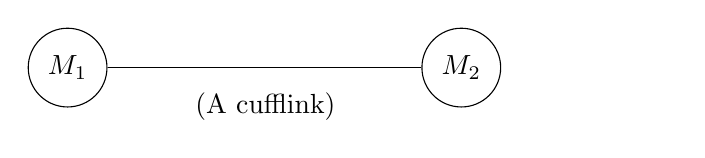
\begin{tikzpicture}
	\node[circle,draw, minimum size=1cm] (M1) at (0,0) {$M_1$};
	\node[circle,draw, minimum size=1cm] (M2) at (5,0) {$M_2$};
	\draw (M1) -- (M2);
	\node[text width=6cm, anchor=west, right] at (1.5,-.5) {(A cufflink)};
	\end{tikzpicture}
\end{center}

The weights of the two ends, $M_1$ and $M_2$ are $i.i.d\ N(5,10)$ 
We want to only keep cufflinks that are balanced. 
That means $\lvert M_{1} - M_{2} \rvert$ is small.

\textbf{A}. It's easy to weigh both ends, $M_{1}+M_{2}$. 
Does this help identify the bad cufflinks?

\textcolor{Red}{No. $M_{1}+M_{2}$ and $M_{1}-M_{2}$ are independent. 
	This is because: 
	$$\begin{aligned}
	\cov [M_{1}+M_{2}, M_{1}-M_{2}] = \var [M_{1}]-\var [M_{2}] = 0
	\end{aligned}$$ }

\textbf{B}. What is the distribution of $M_{1}$ among cufflinks with 
$M_{1}+M_{2}\approx 12$? 

\textcolor{Red}{Let $A=M_{1}+M_{2}$ and $B=M_{1}-M_{2}$, then 
$M_{1}=\frac{A+B}{2}$. 
	From Part A we know $A$ and $B$ are independent. 
	$$\begin{aligned}
	(M_{1}\vert A=12) \stackrel{d}{=} \dfrac{12 + B}{2} \sim N(6,2)
	\end{aligned}$$
	This result follows from the fact that: 
	$$\begin{aligned}
	B \sim N(0,2)
	\end{aligned}$$ 
	Since $B=M_{1}-M_{2}$.
}


\section{Conditional Distributions}

\begin{lemma}[Conditional Distributions]
	Let $\underset{n\times n}{X}$ and $\underset{m\times m}{Y}$ be jointly 
	Gaussian with mean zero and covariance: 
	
	$$\begin{aligned}
	\begin{bmatrix}
	\underset{n\times n}{\Sigma_{XX}} & \underset{m\times n}{\Sigma_{XY}} \\ 
	\underset{n\times m}{\Sigma_{XY}^\intercal}& \underset{m\times 
	m}{\Sigma_{YY}}
	\end{bmatrix}
	\end{aligned}$$
	
	\begin{note} 
		If $\Sigma_{YY}$ is not invertible we can use the Moore-Penrose 
		inverse. 
		The following equations will remain true if the inverse used is the 
		Moore-Penrose generalized inverse.
	\end{note} 
	
	Then, 
	$$\begin{aligned}
	\E[X\vert Y] = \Sigma_{XY}\Sigma_{YY}^{-1} Y
	\end{aligned}$$
	and 
	$$\begin{aligned}
	(X\vert Y=y) \sim N(\Sigma_{XY}\Sigma_{YY}^{-1}y, 
	\Sigma_{XX}-\Sigma_{XY}\Sigma_{YY}^{-1}\Sigma_{XY}^\intercal)
	\end{aligned}$$
	
	\begin{note}
		$\Sigma_{XX}-\Sigma_{XY}\Sigma_{YY}^{-1}\Sigma_{XY}^\intercal$ is the 
		Schur complement of our covariance matrix.
	\end{note}
\end{lemma}



\begin{proof}[]
	Let $A = \Sigma_{XY}\Sigma_{YY}^{-1}Y$ and $X = A+B$. 
	Claim: $B$ is independent of $Y$. 
	$$\begin{aligned}
	\cov[X-\Sigma_{XX}\Sigma_{YY}^{-1}Y,Y] = \cov[X,Y] 
	= \cov[X,Y]-\Sigma_{XY}\Sigma_{YY}^{-1}\cov[Y,Y]  
	= 0 
	\end{aligned}$$
	Now we can say: 
	$$\begin{aligned}
	(X\vert Y=y) \stackrel{d}{=} \Sigma_{XY}\Sigma_{YY}^{-1}y+B 
	\end{aligned}$$
	To confirm that this is the same distribution as before we need to 
	calculate: 
	$$\begin{aligned}
	\cov[B,B] = \cov[X-\Sigma_{XY}\Sigma_{YY}^{-1}Y, 
	X-\Sigma_{XY}\Sigma_{YY}^{-1}Y] \\
	= \cov[X,X] - \cov[X,Y]\Sigma_{YY}^{-1}\Sigma_{XY}^\intercal - 
	\Sigma_{XY}\Sigma_{YY}^{-1}\cov[Y,X] + \Sigma_{XY}\Sigma_{YY}^{-1} 
	\cov[Y,Y]\Sigma_{YY}^{-1}\Sigma_{XY}^\intercal \\= 
	\Sigma_{XX}-\Sigma_{XY}\Sigma_{YY}^{-1}\Sigma_{XY}^\intercal
	\end{aligned}$$
	Thus, $(X\vert Y=y)\sim N(\Sigma_{XY}\Sigma_{YY}^{-1}y,  
	\Sigma_{XX}-\Sigma_{XY}\Sigma_{YY}^{-1}\Sigma_{XY}^\intercal)$
\end{proof}

\section{Gaussian Process Regression}
Suppose we have a random curve that is drawn from a Gaussian process. 
We observe the value of this process at a few noisy points. 
\begin{center}
	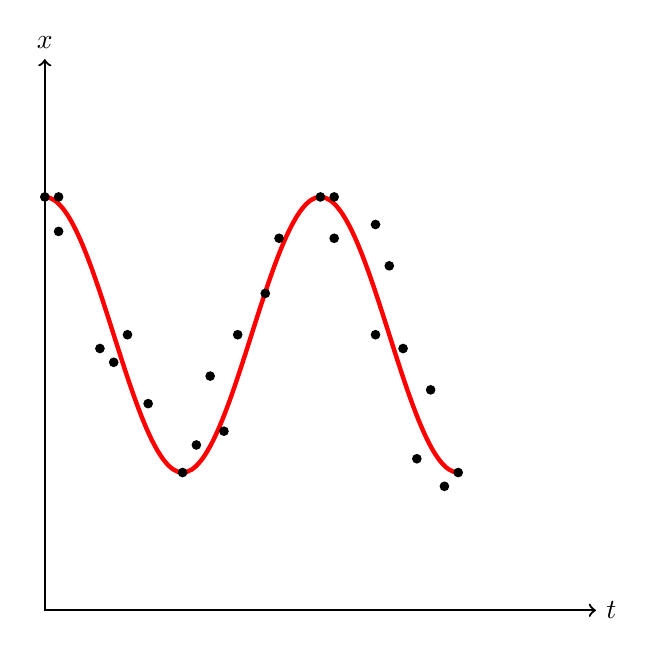
\begin{tikzpicture}[scale=1.75]
	\draw [<->,thick] (0,2) node (yaxis) [above] {$x$}|- (4,-2) node (xaxis) 
	[right] {$t$};
	\draw[x=0.5cm,y=1cm, ultra thick, red](0,1) cos (1,0) sin (2,-1) cos (3,0) 
	sin (4,1) cos (5,0) sin (6,-1);
	
	
	\foreach \point in 
	{(0,1),(.1,1),(.1,.75),(.6,0),(.4,-.1),(.5,-.2),(.75,-.5),(1,-1),(1.1,-.8),(1.2,-.3),(1.3,-.7),(1.4,0),(1.6,.3),(1.7,.7),
	 (2,1), (2.1,1), (2.1,.7), (2.4,0), (2.4,.8), 
	(2.5,.5),(2.6,-.1),(2.7,-.9),(2.8,-.4),(2.9,-1.1),(3,-1)}{% points
		\fill \point circle (1pt);
	}
	\end{tikzpicture}
\end{center}
Using this information we can find out more about this curve, 
including confidence intervals about points. 

But, first we'll look more at the Brownian Bridge. 
Recall (for $0\leq t < 1$), 

$$\begin{aligned}
U_{t} = (B_{t}\vert B_{1}=0) \stackrel{d}{=} B_{t} - tB_{1} 
\end{aligned}$$

Check this, 
$$\begin{aligned}
\cov[B_{1}, B_{t}-tB_{1}]= t - t\cdot 1 = 0 
\end{aligned}$$

Recall, 
$$\begin{aligned}
U_{t}=B_{t}-Z_{0,0}\int_{0}^{t}h_{0}(s)ds=Z(\mathbf{1}_{[0,t)})) - tZ_{0,0} = 
\sum_{n\geq1}\sum_{k=1}^{2^n}Z_{n,k}\int_{0}^{t} h_{n,k}(s)ds
\end{aligned}$$

What is the distribution of $U_{t}-U_{s}$ ? (for $s<t$)
$$\begin{aligned}
U_{t}-U_{s} = \sum_{n\geq1}\sum_{k=1}^{2^n} Z_{n,k}\int_{s}^{t} h_{n,k}(s)ds = 
Z(\mathbf{1}_{[s,t)})-(t-s)Z_{0,0}
\end{aligned}$$
So, 
$$\begin{aligned}
\var[U_{t}-U_{s}] = \var[Z(\mathbf{1}_{[s,t)})]- 
2(t-s)\cdot\cov[Z(\mathbf{1}_{[s,t)}),Z(\mathbf{1}_{[0,1)})] + (t-s)^2 \cdot 
\var[Z(\mathbf{1}_{[0,1)})]
\end{aligned}$$
Note that, 
$$\begin{aligned}
\var[Z(\mathbf{1}_{[s,t)})] = \int_{0}^{1} \mathbf{1}_{[s,t)}(u) \cdot 
\mathbf{1}_{[s,t)}(u) du = t-s 
\end{aligned}$$
So, we'll have 
$$\begin{aligned}
\var[U_{t}-U_{s}] = (t-s) - 2(t-s)^2 + (t-s)^2 = (t-s)[1-(t-s)]
\end{aligned}$$
Thus, 
$$\begin{aligned}
U_{t}-U_{s} \sim N\Big(0, (t-s)[1-(t-s)]\Big)
\end{aligned}$$


\section{Another Application}
Sediment decomposition: 
Let $S_{k}$ = (amount of sediment deposited in year $k$) for $0\leq K \leq 
N=10^4$ 
and we model: 
$$\begin{aligned}
S_{k+1} = \mu + (1-a) \cdot [S_{k}-\mu] + \eta_{k+1}
\end{aligned}$$
we could also write this as: 
$$\begin{aligned}
[S_{k+1}\vert S_{k} \sim N\big((1-a) \cdot [S_{k}-\mu], \sigma^2\big)]
\end{aligned}$$
Here $\eta_{k+1} \sim i.i.d N(0, \sigma^{2})$ where $\sigma^{2} = 10^{-4}$, and 
$a=10^{-3}$
So, $S_{k}$ with $\mu=0$ would look something like this: 
\begin{figure}[H]
	\centering
	\includegraphics[width=0.7\linewidth]{process}
	\caption*{}
	\label{fig:process}
\end{figure}
As shown this is a process that stays distributed about a mean. 

Suppose we have noisy observations of $S_{t}$ for a few years 
Let $Y_{i}$ be our measurements 
$$\begin{aligned}
Y_{i} = S_{k_{i}} + \varepsilon_{i}  
\end{aligned}$$
For $1 \leq i \leq N$ and $\varepsilon_{i} \sim i.i.d N(0, 
\sigma_{\varepsilon}^2)$ 
Our Goal: Estimate the total amount of sediment deposited 
$$\begin{aligned}
S_{\mathrm{total}} = \sum_{k=1}^{N} S_{k}   
\end{aligned}$$
Let $D_{k} = S_{k}-\mu$ we can rewrite this as: 
$$\begin{aligned}
D_{k} = \eta_{k} + (1-a)D_{k-1} =  \eta_{k} + (1-a)\eta_{k-1} + (1-a)^2 D_{k-2} 
= \sum_{j\geq0}(1-a)^j \eta_{k-j}
\end{aligned}$$
Thus, we know: 
$$\begin{aligned}
D_{k}\sim N\bigg(0, \sigma^2 \cdot \sum_{j\geq0}(1-a)^2j\bigg) = N\bigg(0, 
\sigma^2 \dfrac{1}{(2-a)a}\bigg)
\end{aligned}$$
And since $\sigma^2 = 10^{-4}$ and $a=10^{-3}$ we can simplify this further, 
$D_{k} \sim N(0, \sim0.05)$. 
Let's say that $(W_{t})_{t\in\mathbb{R}}$ is a Brownian motion 
and $\eta_{k}= W_\frac{{k+1}}{N} - W_\frac{{k}}{N} \sim N\big(0, 
\frac{1}{N}=\sigma^2\big)$
Then, 
$$\begin{aligned}
D_{k}= \sum_{j\geq0} (1-a)^j \Big(W_\frac{{k-j+1}}{N} - W_\frac{{k-j}}{N} \Big) 
\approx \sum_{j\geq0} e^{-aj} \Big(W_\frac{{k-j+1}}{N} - W_\frac{{k-j}}{N} 
\Big) = \int_{-\infty}^{t} e^{-aN(t-s)}dW_{s}
\end{aligned}$$
Where, $t=\frac{k}{N}$ and $0\leq t \leq 1$ 
Further simplifying we get, 
$$\begin{aligned}
D_{k}= \int_{-\infty}^{t} e^{-aN(t-s)}dW_{s} \sim N(0, 
\int_{-\infty}^{t}(e^{-aN(t-s)})^2 ds = \frac{1}{2aN}) \approx 
\frac{\sigma^2}{2a} + \mathcal{O}(a^2\sigma^2)
\end{aligned}$$
Let $U_{t} = \int_{-\infty}^{t} e^{-aN(t-s)} dW_{s}$ 
Also, $S_{\mathrm{total}}\simeq N\mu + \sum_{k=1}^{N} U_{\frac{k}{N}} \sim 
N\cdot(\mu + \int_{0}^{1}U_{t}dt)$

New question: Let $T=\int_{0}^{1} U_{t}dt$ 
and $X_{i} = U_{t_{i}} + \varepsilon_{i}$ where $\varepsilon_{i}\sim i.i.d 
N(0,\sigma_{\varepsilon}^2)$ 
What is the conditional distribution of $(T\vert X=X_{1},\dotso, X_{N}=X_{N})$ 
? 

Now, we are trying to estimate the total integral, or the purple area below. 
\begin{figure}[H]
	\centering
	\includegraphics[width=0.7\linewidth]{area2}
	\caption*{}
	\label{fig:area2}
\end{figure}
The points on the blue curve are values of $U_{t}$, 
and the purple area is: $\int_{0}^{1} U_{t}dt = T$ 
To do this we need everything inside to be jointly Gaussian. 
i.e. we need to use the same white noise. 

Using the lemma from last lecture, 
we only need their covariance to calculate this area.
Recall the lemma,
if $(X,Y)$ is $N\Bigg(0, \begin{bmatrix} \Sigma_{XX}' & \Sigma_{XY} \\ 
\Sigma_{YX} & \Sigma_{YY}\end{bmatrix}\Bigg)$
then, $(X\vert Y=y) \sim N(\Sigma_{XY}\Sigma_{YY}^{-1}y, 
\Sigma_{XX}-\Sigma_{XY}\Sigma_{YY}^{-1}\Sigma_{XY}^{\intercal})$
To apply this we first need to expand $T$ 
$$\begin{aligned}
T = \int_{0}^{1} U_{t}dt = \int_{0}^{1}\int_{-\infty}^{t} e^{-aN(t-s)} dW_{s}dt 
=\int_{-\infty}^{1}\int_{\max(s,0)}^{t} e^{-aN(t-s)} dtdW_{s}\\
=\int_{-\infty}^{1} 
\frac{1}{aN}e^{aN\min(0,s)}\big(1-e^{-aN}\big)dW_{s}\coloneqq 
\int_{-\infty}^{1}\varphi(s)dW_{s}
\end{aligned}$$ 
Now, we know the following: 
$$\begin{aligned}
\var[T] = \int_{-\infty}^{1} \varphi^{2}(s) ds 
\end{aligned}$$ 

$$\begin{aligned}
\var[X_{i}] = \var[U_{t_{i}}] + \sigma_{\varepsilon} = \frac{1}{2aN} + 
\sigma_{\varepsilon}^2 
\end{aligned}$$ 

$$\begin{aligned}
\cov[X_{i}, X_{j}] = \int_{-\infty}^{t_{i}}e^{-aN(t_{i}-s)}\cdot 
e^{-aN(t_{j}-s)} ds = \frac{1}{2aN}[e^{-aN(t_{j}-t_{i})}]
\end{aligned}$$

for $i\neq j$ and $t_{i}<t_{j}$ 
Thus, 
$$\begin{aligned}
\cov[X_{i}, T] = \int_{-\infty}^{t} e^{-aN(t_{i}-s)}\varphi(s) ds 
\end{aligned}$$
where, 
$$\begin{aligned}
\Sigma = 
\begin{bmatrix}
&  &  &  &  \\
\vert\vert\varphi^2\vert\vert & 0 & \dotso & \dotso & 0 \\
0 & \frac{1}{2aN}+\varepsilon^2 & 0 & \dotso & 0 \\
0 & 0 & \ddots & \hfill & 0\\
\vdots & \vdots & \vdots & \ddots & \vdots \\
0 & 0 & 0 & 0 & \frac{1}{2aN}+\varepsilon^2
\end{bmatrix}
\end{aligned}$$
Where the columns are associated with $T$, $X_{1}$, $X_{2}$, and so forth. 
And the rows are similarly associated with $T$, $X_{1}$, $X_{2}$, and so forth. 
(This means the diagonal elements are the variances of $T$, $X_{1}$, $X_{2}$, 
$\dotso$, $X_N$).
% ==============================================================================
%
\end{document}
%
% ==============================================================================
